\documentclass[a4paper]{report}
\usepackage[utf8]{inputenc}
\usepackage[portuguese]{babel}
\usepackage{hyperref}
\usepackage{a4wide}
\hypersetup{pdftitle={VC - Turorial 1},
pdfauthor={José Ferreira, Luís Pereira},
colorlinks=true,
urlcolor=blue,
linkcolor=black}
\usepackage{subcaption}
\usepackage{listings}
\usepackage{booktabs}
\usepackage{multirow}
\usepackage{appendix}
\usepackage{tikz}
\usepackage{authblk}
\usepackage{bashful}
\usepackage{verbatim}
\usepackage{amssymb}
\usepackage{multirow}
\usepackage{mwe}
\usepackage{float}
\usetikzlibrary{positioning,automata,decorations.markings}
\AfterEndEnvironment{figure}{\noindent\ignorespaces}
\AfterEndEnvironment{table}{\noindent\ignorespaces}

\begin{document}

\title{VC - Turorial 1}
\author{José Ferreira (A83683), Luís Pereira (A86265}
\date{\today}

\begin{center}
    \begin{minipage}{0.75\linewidth}
        \centering
        
\includegraphics[width=0.4\textwidth]{images/eng.jpeg}\par\vspace{1cm}
        \vspace{1.5cm}
        \href{https://www.uminho.pt/PT}
        {\color{black}{\scshape\LARGE Universidade do Minho}} \par
        \vspace{1cm}
        \href{https://www.di.uminho.pt/}
        {\color{black}{\scshape\Large Departamento de Informática}} \par
        \vspace{1.5cm}
        \maketitle
    \end{minipage}
\end{center}

\tableofcontents

\pagebreak
\chapter{Introdução}

\chapter{Exercício 1 - Smooth Images}
\section{Ruído}
Para introduzir ruído numa imagem foi criado uma função denominada de ruído.
Esta recebe uma matriz que representa uma imagem, o tipo de ruído a ser
utilizado e os parâmetros para esse ruído. Caso o tipo de ruído escolhido seja
\textit{gaussian} o parâmetro representa a variância, caso o ruído seja
\textit{salt-n-pepper} o parâmetro representa a percentagem de ocorrência.

\begin{figure}[H]
    \centering
    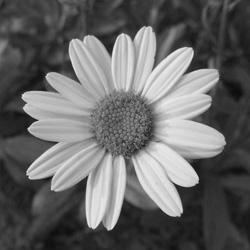
\includegraphics[width=0.5\textwidth]{images/flower.jpg}
    \caption{Imagem Original}
\end{figure}

\begin{figure}[H]
    \centering
    \begin{minipage}{.5\textwidth}
        \centering
        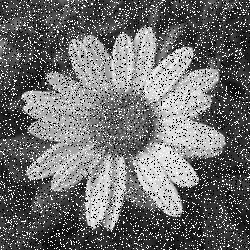
\includegraphics[width=0.95\textwidth]{images/flower_salt-n-pepper_0.2.png}
        \captionof{figure}{Salt-n-pepper com ocorrência de 0.2}
    \end{minipage}%
    \begin{minipage}{.5\textwidth}
        \centering
        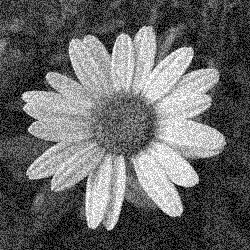
\includegraphics[width=0.95\textwidth]{images/flower_gaussian_0.2.png}
        \captionof{figure}{Gaussiano com variância 0.2}
    \end{minipage}
\end{figure}

\chapter{Exercicio 2 - Detect Edges}

\end{document}
